\documentclass[aspectratio=169,10pt]{beamer}
\usetheme{metropolis}
\usepackage{amsmath,amssymb,braket}
\usepackage{tikz}
\usetikzlibrary{positioning,arrows.meta,shapes.geometric,calc,decorations.pathreplacing,fit,backgrounds,matrix}
\usepackage{xcolor}
\usepackage{array}
\usepackage{listings}
\usepackage{appendixnumberbeamer}

% ── Color scheme (matches presentation20260208.tex) ──
\definecolor{leangreen}{RGB}{34,180,34}
\definecolor{leanblue}{RGB}{70,130,180}
\definecolor{amber}{RGB}{255,191,0}
\definecolor{softred}{RGB}{220,80,80}
\definecolor{darkbg}{RGB}{15,15,15}
\definecolor{cardbg}{RGB}{30,30,30}
\definecolor{dimwhite}{RGB}{180,180,180}

\setbeamercolor{background canvas}{bg=darkbg}
\setbeamercolor{normal text}{fg=white}
\setbeamercolor{title}{fg=white}
\setbeamercolor{frametitle}{fg=white,bg=darkbg}
\setbeamercolor{block title}{fg=white,bg=gray!30!black}
\setbeamercolor{block body}{fg=white,bg=cardbg}
\setbeamercolor{alerted text}{fg=amber}
\setbeamercolor{example text}{fg=leangreen}
\setbeamercolor{itemize item}{fg=leangreen}
\setbeamercolor{itemize subitem}{fg=dimwhite}
\setbeamercolor{enumerate item}{fg=leangreen}
\setbeamercolor{progress bar}{fg=leangreen}
\setbeamercolor{title separator}{fg=leangreen}
\setbeamercolor{footline}{fg=dimwhite,bg=darkbg}

% ── Footer with page number / total ──
\setbeamertemplate{footline}{%
  \hfill%
  \usebeamercolor[fg]{footline}%
  \usebeamerfont{footline}%
  \insertframenumber\,/\,\inserttotalframenumber%
  \hspace*{6pt}\par%
}

% ── Lean listing ──
\lstdefinelanguage{Lean}{
  keywords={theorem, lemma, def, abbrev, variable, namespace, end, open, import,
            noncomputable, private, section, structure, where, let, have, exact,
            intro, apply, simp, rw, rcases, refine, classical, cases, with,
            fun, forall, exists, Prop, Type},
  keywordstyle=\color{leanblue}\bfseries,
  keywords=[2]{IsInjective, SameMPV, SameMPV2, GaugeEquiv, MPSTensor, Matrix, Fin, GL,
               CanonicalForm, AlgEquiv, TwoSidedIdeal, piAlgEquiv, toTensorFromBlocks,
               perBlockLinearExtension, mpv, mpvFun},
  keywordstyle=[2]\color{leangreen},
  comment=[l]{--},
  commentstyle=\color{gray}\itshape,
  string=[b]",
  stringstyle=\color{orange},
  basicstyle=\ttfamily\scriptsize\color{white},
  backgroundcolor=\color{cardbg},
  breaklines=true,
  frame=single,
  rulecolor=\color{gray!50!black},
  showstringspaces=false,
  escapeinside={(*@}{@*)},
}
\lstset{language=Lean}

% ── Macros ──
\newcommand{\proved}[1]{\textcolor{leangreen}{\checkmark\  #1}}
\newcommand{\inprog}[1]{\textcolor{amber}{$\circ$\  #1}}
\newcommand{\future}[1]{\textcolor{gray}{$\diamond$\  #1}}
\newcommand{\notproved}[1]{\textcolor{softred}{$\boldsymbol{\times}$\  #1}}
\newcommand{\MD}{M_D(\mathbb{C})}
\newcommand{\GLC}{\mathrm{GL}}
\newcommand{\tr}{\mathrm{tr}}

\title{\textbf{The One Remaining Gap:\\Separating Block MPVs from Global Equality}}
\subtitle{{\small A detailed analysis of the unformalizable step  $\cdot$  2792 lines $\cdot$ 16 modules $\cdot$ 0 sorries}}
\date{February 9, 2026}
\author{}

\begin{document}

%======================================================================
% SLIDE 1 - Title
%======================================================================
{%
\setbeamertemplate{footline}{}
\begin{frame}[plain,noframenumbering]
\vspace{-2em}
\maketitle
\vspace{-2em}
\begin{center}
{\footnotesize Lean~4 + Mathlib v4.27.0\quad$\cdot$\quad arXiv:2011.12127\quad$\cdot$\quad\texttt{github.com/LionSR/MPSLean}}
\end{center}
\end{frame}
}

%======================================================================
% SLIDE 2 - What We Proved: Architecture Overview
%======================================================================
\begin{frame}{What We Proved: The Full Architecture}
\vspace{-0.4em}
\begin{center}
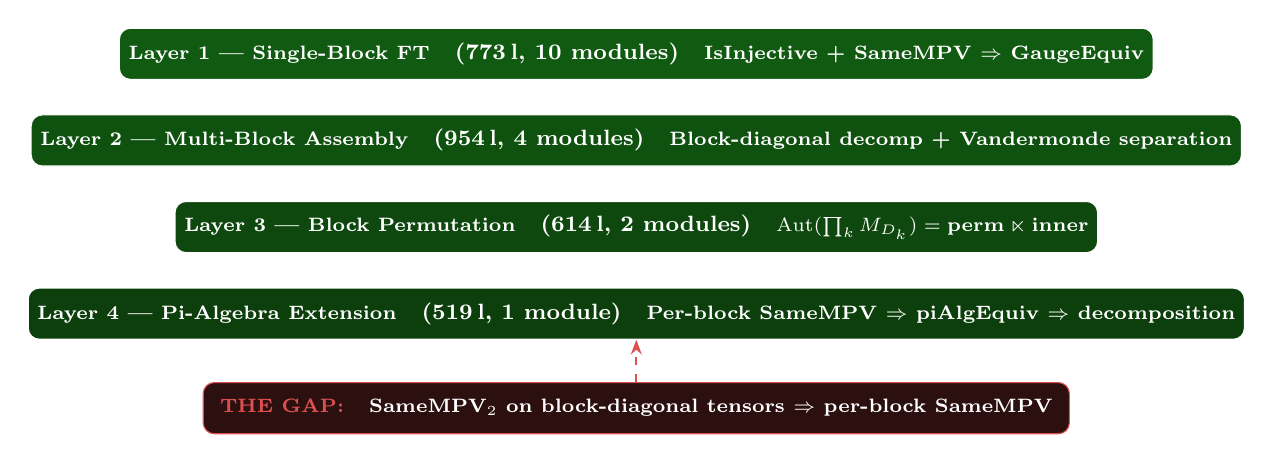
\begin{tikzpicture}[xscale=0.95,
  layer/.style={rectangle,rounded corners,draw=white,text=white,
    font=\scriptsize\bfseries,minimum width=11cm,minimum height=0.65cm,align=center},
  arr/.style={-{Stealth[scale=0.8]},white,thick}
]
\node[layer,fill=leangreen!50!black] (L1) at (0,3.0) {
  \textbf{Layer 1 --- Single-Block FT}\quad{\footnotesize(773\,l, 10 modules)}\quad
  IsInjective + SameMPV $\Rightarrow$ GaugeEquiv};
\node[layer,fill=leangreen!45!black] (L2) at (0,1.9) {
  \textbf{Layer 2 --- Multi-Block Assembly}\quad{\footnotesize(954\,l, 4 modules)}\quad
  Block-diagonal decomp + Vandermonde separation};
\node[layer,fill=leangreen!40!black] (L3) at (0,0.8) {
  \textbf{Layer 3 --- Block Permutation}\quad{\footnotesize(614\,l, 2 modules)}\quad
  $\mathrm{Aut}(\prod_k M_{D_k}) = \text{perm} \ltimes \text{inner}$};
\node[layer,fill=leangreen!35!black] (L4) at (0,-0.3) {
  \textbf{Layer 4 --- Pi-Algebra Extension}\quad{\footnotesize(519\,l, 1 module)}\quad
  Per-block SameMPV $\Rightarrow$ piAlgEquiv $\Rightarrow$ decomposition};
\draw[arr] (L1) -- (L2);
\draw[arr] (L2) -- (L3);
\draw[arr] (L3) -- (L4);

% The gap annotation
\node[rectangle,rounded corners,draw=softred,fill=softred!20!black,text=white,
  font=\scriptsize\bfseries,minimum width=11cm,minimum height=0.65cm,align=center]
  (GAP) at (0,-1.5) {
  \textcolor{softred}{\textbf{THE GAP:}}\quad
  SameMPV${}_2$ on block-diagonal tensors $\Rightarrow$ per-block SameMPV};
\draw[-{Stealth[scale=0.8]},softred,thick,dashed] (GAP) -- (L4);
\end{tikzpicture}
\end{center}

\vspace{0.1em}
{\small \textbf{Score:} \textcolor{leangreen}{2792 lines, 16 modules, 0 sorries, 0 axioms.}\quad
The gap is \emph{not} a sorry --- it's a hypothesis we can't yet derive.}
\end{frame}

%======================================================================
% SLIDE 3 - What We Proved: Key Results
%======================================================================
\begin{frame}[fragile]{What We Proved: Key Theorems in Lean}
\vspace{-0.4em}
\begin{columns}[T]
\column{0.48\textwidth}
{\small\textbf{\textcolor{leangreen}{Single-block:}}}
\begin{lstlisting}[basicstyle=\ttfamily\fontsize{5.5}{7}\selectfont\color{white}]
theorem fundamentalTheorem_singleBlock
    {A B : MPSTensor d D}
    (hA : IsInjective A)
    (hAB : SameMPV A B) :
    GaugeEquiv A B
\end{lstlisting}

\vspace{0.3em}
{\small\textbf{\textcolor{leangreen}{Multi-block (from per-block):}}}
\begin{lstlisting}[basicstyle=\ttfamily\fontsize{5.5}{7}\selectfont\color{white}]
theorem fundamentalTheorem_multiBlock_full
    ((*@$\mu$@*) : Fin r (*@$\to$@*) (*@$\mathbb{C}$@*))
    (A B : (k : Fin r) (*@$\to$@*) MPSTensor d (dim k))
    (hA : (*@$\forall$@*) k, IsInjective (A k))
    (hSame : (*@$\forall$@*) k, SameMPV (A k) (B k)) :
    ((*@$\forall$@*) k, GaugeEquiv (A k) (B k)) (*@$\wedge$@*)
    GaugeEquiv (toTensorFromBlocks (*@$\mu$@*) A)
               (toTensorFromBlocks (*@$\mu$@*) B)
\end{lstlisting}

\column{0.48\textwidth}
{\small\textbf{\textcolor{leangreen}{Forward direction (proved):}}}
\begin{lstlisting}[basicstyle=\ttfamily\fontsize{5.5}{7}\selectfont\color{white}]
theorem sameMPV2_summed_blocks
    ((*@$\mu$@*) : Fin r (*@$\to$@*) (*@$\mathbb{C}$@*))
    (A B : (k : Fin r) (*@$\to$@*) MPSTensor d (dim k))
    (hSame : SameMPV2
      (toTensorFromBlocks (*@$\mu$@*) A)
      (toTensorFromBlocks (*@$\mu$@*) B))
    (N : (*@$\mathbb{N}$@*)) ((*@$\sigma$@*) : Fin N (*@$\to$@*) Fin d) :
    (*@$\sum$@*) k, ((*@$\mu$@*) k) ^ N (*@$\bullet$@*) mpv (A k) (*@$\sigma$@*)
    = (*@$\sum$@*) k, ((*@$\mu$@*) k) ^ N (*@$\bullet$@*) mpv (B k) (*@$\sigma$@*)
\end{lstlisting}

\vspace{0.2em}
{\small\textbf{\textcolor{softred}{The gap (not proved):}}}
\begin{lstlisting}[basicstyle=\ttfamily\fontsize{5.5}{7}\selectfont\color{white}]
-- NOT FORMALIZED:
-- SameMPV2 on block-diagonal tensors
-- (*@$\Rightarrow$@*) (*@$\forall$@*) k, SameMPV (A k) (B k)
\end{lstlisting}
\end{columns}
\end{frame}

%======================================================================
% SLIDE 4 - The Gap: Precise Statement
%======================================================================
\begin{frame}{The Gap: Precise Mathematical Statement}
\vspace{-0.5em}
\begin{block}{What we have (proved --- \texttt{sameMPV${}_2$\_summed\_blocks})}
\vspace{-0.6em}
\[
\forall\, N\in\mathbb{N},\; \forall\,\sigma\!: \mathrm{Fin}\,N \to \mathrm{Fin}\,d:\quad
\sum_{k=1}^{r} \mu_k^N \cdot \mathrm{mpv}(A_k, \sigma) = 
\sum_{k=1}^{r} \mu_k^N \cdot \mathrm{mpv}(B_k, \sigma)
\]
\vspace{-0.8em}
\end{block}
\vspace{-0.2em}
\begin{block}{What we want (not proved)}
\vspace{-0.6em}
\[
\forall\, k,\; \forall\, N\in\mathbb{N},\; \forall\,\sigma\!: \mathrm{Fin}\,N \to \mathrm{Fin}\,d:\quad
\mathrm{mpv}(A_k, \sigma) =  \mathrm{mpv}(B_k, \sigma)
\]
\vspace{-0.8em}
\end{block}

\vspace{0.1em}
{\small Define $\delta_k(N, \sigma) :=  \mathrm{mpv}(A_k, \sigma) - \mathrm{mpv}(B_k, \sigma)$.}

\vspace{0.15em}
{\small \textbf{Have:} $\sum_{k=1}^r \mu_k^N \cdot \delta_k(N, \sigma) = 0$ for all $N$ and $\sigma : \mathrm{Fin}\,N \to \mathrm{Fin}\,d$.}

\vspace{0.05em}
{\small \textbf{Want:} $\delta_k(N, \sigma) = 0$ for all $k$, $N$, $\sigma$.}

\vspace{0.2em}
{\small At first glance, this looks like Vandermonde invertibility. It is not.}
\end{frame}

%======================================================================
% SLIDE 5 - Background: What is a Vandermonde Matrix?
%======================================================================
\begin{frame}{Background: What Is a Vandermonde Matrix?}
\vspace{-0.3em}
{\small Given \textbf{distinct} scalars $\mu_1, \dots, \mu_r$, the \textbf{Vandermonde matrix} is:}
\[
V = \begin{pmatrix}
1 & 1 & \cdots & 1 \\
\mu_1 & \mu_2 & \cdots & \mu_r \\
\mu_1^2 & \mu_2^2 & \cdots & \mu_r^2 \\
\vdots & \vdots & \ddots & \vdots \\
\mu_1^{r-1} & \mu_2^{r-1} & \cdots & \mu_r^{r-1}
\end{pmatrix}
\qquad\text{i.e., } V_{N,k} = \mu_k^N
\]

\vspace{-0.2em}
\begin{columns}[T]
\column{0.52\textwidth}
{\small\textbf{Concrete example} ($\mu_1 = 2, \mu_2 = 3, \mu_3 = 5$):}
\[
V = \begin{pmatrix}
1 & 1 & 1 \\
2 & 3 & 5 \\
4 & 9 & 25
\end{pmatrix}
\quad \det V = 6 \neq 0
\]

\column{0.44\textwidth}
{\small\textbf{Key theorem} (known since 1830s):}
\[
\det V = \prod_{1 \leq i < j \leq r} (\mu_j - \mu_i)
\]

\vspace{0.2em}
{\small This is $\neq 0$ \textbf{if and only if} all $\mu_k$ are distinct.}
\end{columns}

\vspace{0.5em}
{\small\textbf{Intuition:} Each column of $V$ records the powers of a different base. When the bases are distinct, these ``exponential signatures'' are linearly independent --- no column can be written as a combination of the others.}
\end{frame}

%======================================================================
% SLIDE 6 - Why Vandermonde Matrices Matter Here
%======================================================================
\begin{frame}{Why Vandermonde Matrices Matter for Our Problem}
\vspace{-0.5em}
{\small\textbf{The key consequence:} If $V$ is invertible, $V \cdot c = 0$ has \textbf{only} the trivial solution $c = 0$.}

\vspace{0.1em}
\begin{center}
\begin{tikzpicture}[scale=0.55]
% Vandermonde matrix
\draw[white,thick] (0,0) rectangle (4,3.2);
\foreach \j [evaluate=\j as \jj using int(\j+1)] in {0,1,2,3} {
  \node[font=\tiny,white] at (\j+0.5,2.7) {$\mu_{\jj}^0$};
  \node[font=\tiny,white] at (\j+0.5,1.95) {$\mu_{\jj}^1$};
  \node[font=\tiny,white] at (\j+0.5,1.2) {$\mu_{\jj}^2$};
  \node[font=\tiny,white] at (\j+0.5,0.45) {$\mu_{\jj}^3$};
}
\draw[white,thin] (0,2.4) -- (4,2.4);
\draw[white,thin] (0,1.65) -- (4,1.65);
\draw[white,thin] (0,0.9) -- (4,0.9);
\draw[white,thin] (1,0) -- (1,3.2);
\draw[white,thin] (2,0) -- (2,3.2);
\draw[white,thin] (3,0) -- (3,3.2);
% Times vector
\node[font=\normalsize,white] at (4.7,1.6) {$\cdot$};
\draw[white,thick] (5.2,0.4) rectangle (6,2.8);
\node[font=\tiny,white] at (5.6,2.35) {$c_1$};
\node[font=\tiny,white] at (5.6,1.75) {$c_2$};
\node[font=\tiny,white] at (5.6,1.15) {$c_3$};
\node[font=\tiny,white] at (5.6,0.55) {$c_4$};
% Equals zero
\node[font=\normalsize,white] at (6.7,1.6) {$=$};
\draw[white,thick] (7.2,0.4) rectangle (8,2.8);
\node[font=\tiny,white] at (7.6,2.35) {$0$};
\node[font=\tiny,white] at (7.6,1.75) {$0$};
\node[font=\tiny,white] at (7.6,1.15) {$0$};
\node[font=\tiny,white] at (7.6,0.55) {$0$};
% Arrow
\node[font=\large,leangreen] at (9.5,1.6) {$\Longrightarrow$};
\node[font=\footnotesize,leangreen,right] at (10.2,1.6) {$c_k = 0\ \forall k$};
\end{tikzpicture}
\end{center}

\vspace{-0.3em}
{\small\textbf{In plain English:} If someone tells you
$c_1 \cdot \mu_1^N + c_2 \cdot \mu_2^N + \cdots + c_r \cdot \mu_r^N = 0$
for $N = 0, 1, \dots, r{-}1$ and the $\mu_k$ are all different, then every $c_k = 0$. Distinct exponentials cannot conspire to cancel at $r$ consecutive powers.}

\vspace{0.3em}
\begin{center}
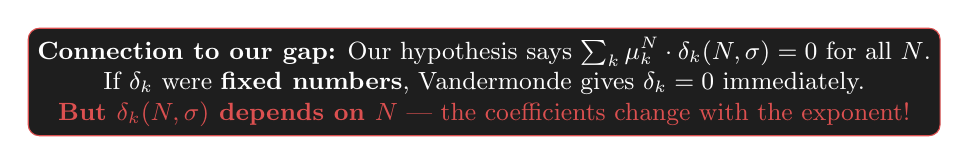
\begin{tikzpicture}
\node[rectangle,rounded corners,draw=softred,fill=cardbg,text=white,
  font=\small,align=center,minimum width=11cm,minimum height=0.7cm] {
  \textbf{Connection to our gap:} Our hypothesis says $\sum_k \mu_k^N \cdot \delta_k(N,\sigma) = 0$ for all $N$.\\
  If $\delta_k$ were \textbf{fixed numbers}, Vandermonde gives $\delta_k = 0$ immediately.\\
  \textcolor{softred}{\textbf{But $\delta_k(N,\sigma)$ depends on $N$} --- the coefficients change with the exponent!}
};
\end{tikzpicture}
\end{center}
\end{frame}

%======================================================================
% SLIDE 7 - Why Vandermonde Should Work (our Lean tools)
%======================================================================
\begin{frame}{Our Vandermonde Tools in Lean}
\vspace{-0.3em}
{\small We \emph{have} formalized the Vandermonde argument. It works perfectly when the coefficients are fixed:}

\vspace{0.3em}
{\small\textbf{\textcolor{leangreen}{What we proved:}}}
\begin{itemize}
  \item {\small \texttt{vandermonde\_separation}: wraps Mathlib's \texttt{det\_vandermonde}; if $\mu_k$ distinct and $\sum_k c_k \cdot \mu_k^N = 0$ for $N = 0, \dots, r{-}1$, then $c_k = 0$.}
  \item {\small \texttt{vandermonde\_separation\_fun}: a \textbf{function-valued} generalization. If $v_k : \alpha \to \mathbb{C}$ and $\sum_k v_k(a) \cdot \mu_k^N = 0$ for all $a \in \alpha$ and $N = 0, \dots, r{-}1$, then $v_k = 0$.}
\end{itemize}

\vspace{0.3em}
{\small\textbf{\textcolor{leangreen}{These are used}} in multi-block matching (\texttt{FundamentalTheoremMulti.lean}) to separate blocks at a \emph{fixed} system size.}

\vspace{0.5em}
\begin{center}
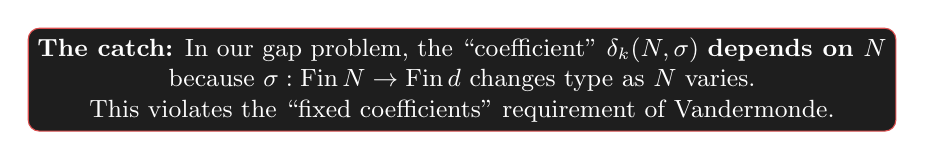
\begin{tikzpicture}
\node[rectangle,rounded corners,draw=softred,fill=cardbg,text=white,
  font=\small,align=center,minimum width=11cm,minimum height=0.9cm] {
  \textbf{The catch:} In our gap problem, the ``coefficient'' $\delta_k(N, \sigma)$ \textbf{depends on $N$}\\
  because $\sigma : \mathrm{Fin}\,N \to \mathrm{Fin}\,d$ changes type as $N$ varies.\\
  This violates the ``fixed coefficients'' requirement of Vandermonde.
};
\end{tikzpicture}
\end{center}
\end{frame}

%======================================================================
% SLIDE 6 - The Type-Level Coupling Problem
%======================================================================
\begin{frame}{The Core Difficulty: Type-Level Coupling of $N$ and $\sigma$}
\vspace{-0.3em}
\begin{columns}[T]
\column{0.52\textwidth}
{\small\textbf{In the standard Vandermonde setting:}}
\begin{itemize}
\item Row index: $N \in \{0, \dots, r{-}1\}$ \textcolor{leangreen}{(varies)}
\item Coefficients: $c_k \in \mathbb{C}$ \textcolor{leangreen}{(fixed!)}
\end{itemize}

\vspace{0.3em}
{\small\textbf{In our MPS setting:}}
\begin{itemize}
\item Exponent: $N \in \mathbb{N}$ \textcolor{leangreen}{(varies)}
\item ``Coefficients'': $\delta_k(N, \sigma)$ \textcolor{softred}{(\textbf{depend on $N$!})}
\item Configuration: $\sigma : \mathrm{Fin}\,N \to \mathrm{Fin}\,d$ \textcolor{softred}{(\textbf{type depends on $N$!})}
\end{itemize}

\column{0.44\textwidth}
\begin{center}
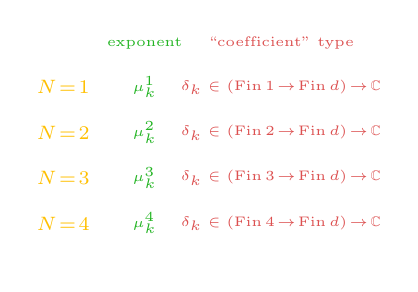
\begin{tikzpicture}[scale=0.72]
% The "matrix" with varying types
\draw[white,thick] (0,0) rectangle (5,3.6);
% Row labels
\node[font=\scriptsize,amber,left] at (0,3.1) {$N\!=\!1$};
\node[font=\scriptsize,amber,left] at (0,2.3) {$N\!=\!2$};
\node[font=\scriptsize,amber,left] at (0,1.5) {$N\!=\!3$};
\node[font=\scriptsize,amber,left] at (0,0.7) {$N\!=\!4$};
% Exponent column
\node[font=\tiny,leangreen] at (0.8,3.1) {$\mu_k^1$};
\node[font=\tiny,leangreen] at (0.8,2.3) {$\mu_k^2$};
\node[font=\tiny,leangreen] at (0.8,1.5) {$\mu_k^3$};
\node[font=\tiny,leangreen] at (0.8,0.7) {$\mu_k^4$};
% Coefficient column
\node[font=\tiny,softred] at (3.2,3.1) {$\delta_k \in (\mathrm{Fin}\,1\!\to\!\mathrm{Fin}\,d)\!\to\!\mathbb{C}$};
\node[font=\tiny,softred] at (3.2,2.3) {$\delta_k \in (\mathrm{Fin}\,2\!\to\!\mathrm{Fin}\,d)\!\to\!\mathbb{C}$};
\node[font=\tiny,softred] at (3.2,1.5) {$\delta_k \in (\mathrm{Fin}\,3\!\to\!\mathrm{Fin}\,d)\!\to\!\mathbb{C}$};
\node[font=\tiny,softred] at (3.2,0.7) {$\delta_k \in (\mathrm{Fin}\,4\!\to\!\mathrm{Fin}\,d)\!\to\!\mathbb{C}$};
% Separator
\draw[white,thin,dashed] (1.5,0) -- (1.5,3.6);
% Labels
\node[font=\tiny,leangreen,above] at (0.8,3.6) {exponent};
\node[font=\tiny,softred,above] at (3.2,3.6) {``coefficient'' type};
\end{tikzpicture}
\end{center}
\end{columns}

\vspace{0.3em}
\begin{center}
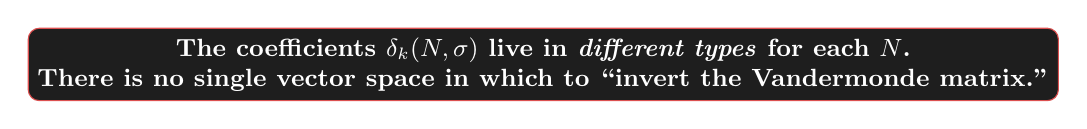
\begin{tikzpicture}
\node[rectangle,rounded corners,draw=softred,fill=cardbg,text=white,
  font=\small,align=center,minimum width=10.5cm,minimum height=0.7cm] {
  \textbf{The coefficients $\delta_k(N,\sigma)$ live in \emph{different types} for each $N$.}\\
  \textbf{There is no single vector space in which to ``invert the Vandermonde matrix.''}
};
\end{tikzpicture}
\end{center}
\end{frame}

%======================================================================
% SLIDE 7 - Diagram: The Coupling Structure
%======================================================================
\begin{frame}{Visualizing the Coupling}
\vspace{-0.5em}
\begin{center}
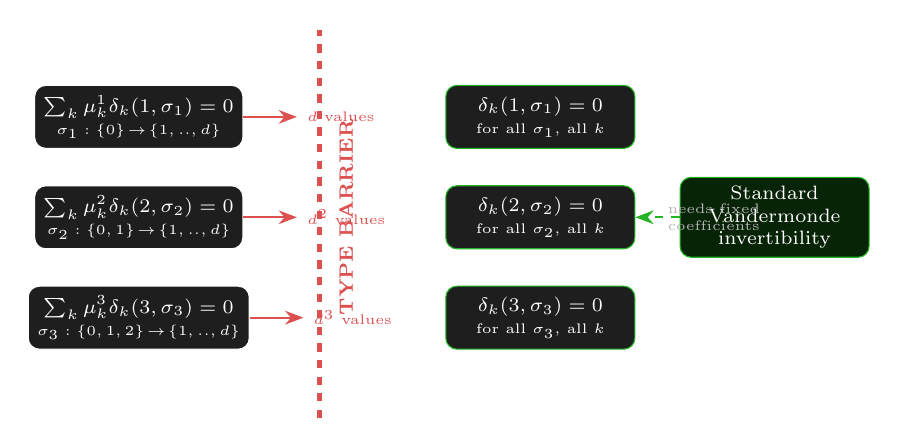
\begin{tikzpicture}[scale=0.85,
  block/.style={rectangle,rounded corners,draw=white,fill=cardbg,text=white,
    font=\scriptsize,minimum width=2.4cm,minimum height=0.8cm,align=center}
]
% Left: what we have
\node[font=\small\bfseries,white] at (-4.5,3.5) {What we have};
\node[block] (eq1) at (-4.5,2.5) {$\sum_k \mu_k^1 \delta_k(1,\sigma_1) = 0$\\
  {\tiny$\sigma_1 : \{0\}\!\to\!\{1,..,d\}$}};
\node[block] (eq2) at (-4.5,1.0) {$\sum_k \mu_k^2 \delta_k(2,\sigma_2) = 0$\\
  {\tiny$\sigma_2 : \{0,1\}\!\to\!\{1,..,d\}$}};
\node[block] (eq3) at (-4.5,-0.5) {$\sum_k \mu_k^3 \delta_k(3,\sigma_3) = 0$\\
  {\tiny$\sigma_3 : \{0,1,2\}\!\to\!\{1,..,d\}$}};
\node[font=\large,white] at (-4.5,-1.5) {$\vdots$};

% Middle: the obstacle
\draw[softred,ultra thick,dashed] (-1.8,-2) -- (-1.8,3.8);
\node[font=\scriptsize\bfseries,softred,rotate=90] at (-1.4,1) {TYPE BARRIER};

% Right: what we want
\node[font=\small\bfseries,white] at (3,3.5) {What we want};
\node[block,draw=leangreen] (w1) at (1.5,2.5) {$\delta_k(1,\sigma_1) = 0$\\{\tiny for all $\sigma_1$, all $k$}};
\node[block,draw=leangreen] (w2) at (1.5,1.0) {$\delta_k(2,\sigma_2) = 0$\\{\tiny for all $\sigma_2$, all $k$}};
\node[block,draw=leangreen] (w3) at (1.5,-0.5) {$\delta_k(3,\sigma_3) = 0$\\{\tiny for all $\sigma_3$, all $k$}};
\node[font=\large,white] at (1.5,-1.5) {$\vdots$};

% Right: standard Vandermonde
\node[block,fill=leangreen!20!black,draw=leangreen] (vand) at (5,1.0) {Standard\\Vandermonde\\invertibility};
\draw[-{Stealth},leangreen,thick,dashed] (vand) -- node[right,font=\tiny,text=dimwhite,align=left]{needs fixed\\coefficients} (w2);

% Arrows showing the problem
\draw[-{Stealth},softred,thick] (eq1.east) -- ++(0.8,0) node[right,font=\tiny,softred] {$d$ values};
\draw[-{Stealth},softred,thick] (eq2.east) -- ++(0.8,0) node[right,font=\tiny,softred] {$d^2$ values};
\draw[-{Stealth},softred,thick] (eq3.east) -- ++(0.8,0) node[right,font=\tiny,softred] {$d^3$ values};

\end{tikzpicture}
\end{center}

\vspace{-0.2em}
{\small\textbf{The issue:} Each row of the ``Vandermonde system'' has $d^N$ equations (one per $\sigma$), but the $\sigma$-spaces for different $N$ are unrelated. We cannot form a single matrix equation $V \cdot c = 0$.}
\end{frame}

%======================================================================
% SLIDE 8 - Approach 1: Standard Vandermonde Across Sizes
%======================================================================
\begin{frame}{Approach 1: Standard Vandermonde Across System Sizes}
\vspace{-0.3em}
{\small\textbf{Idea:} Fix a configuration $\sigma_0$ at size $N_0$, then vary $N$ to get a Vandermonde system.}

\vspace{0.2em}
{\small\textbf{Problem:} Varying $N$ changes the \emph{type} of $\sigma$. We cannot ``hold $\sigma$ fixed'' while varying $N$.}

\vspace{0.3em}
\begin{center}
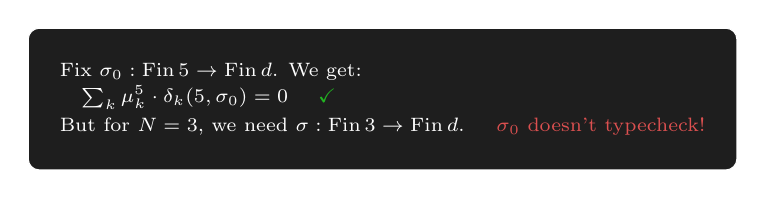
\begin{tikzpicture}[scale=0.8]
\node[rectangle,rounded corners,draw=white,fill=cardbg,text=white,
  font=\scriptsize,minimum width=9cm,minimum height=1.8cm,align=left] {
  Fix $\sigma_0 : \mathrm{Fin}\,5 \to \mathrm{Fin}\,d$. We get:\\[0.2em]
  \quad $\sum_k \mu_k^5 \cdot \delta_k(5, \sigma_0) = 0$ \quad\textcolor{leangreen}{\checkmark}\\[0.3em]
  But for $N = 3$, we need $\sigma : \mathrm{Fin}\,3 \to \mathrm{Fin}\,d$. \quad\textcolor{softred}{$\sigma_0$ doesn't typecheck!}
};
\end{tikzpicture}
\end{center}

\vspace{0.3em}
{\small\textbf{Could we restrict $\sigma_0$?} Truncate $\sigma_0$ to its first 3 components?}

\vspace{0.1em}
{\small Yes, but then $\delta_k(3, \sigma_0|_3)$ and $\delta_k(5, \sigma_0)$ are \emph{different values}. We need the \emph{same} $c_k$ at each row, and we have:}
\[
\delta_k(N, \sigma) = \tr\!(\textstyle\prod_{j=0}^{N-1} A_k^{\sigma(j)}) - \tr\!(\textstyle\prod_{j=0}^{N-1} B_k^{\sigma(j)})
\]

\vspace{-0.2em}
{\small Different $N$ $\Rightarrow$ different product $\Rightarrow$ different trace $\Rightarrow$ different ``coefficient''.}

\vspace{0.3em}
\notproved{Cannot form a Vandermonde system: coefficients depend on row index.}
\end{frame}

%======================================================================
% SLIDE 9 - Approach 2: Word Repetition Trick
%======================================================================
\begin{frame}{Approach 2: The Word Repetition Trick}
\vspace{-0.3em}
{\small\textbf{Idea:} Fix a word $w$ of length $L$. Consider the word $w^m = \underbrace{w \cdots w}_{m\text{ times}}$.}

\vspace{0.1em}
{\small Then $\mathrm{mpv}(A_k, w^m) = \tr((\mathrm{eval}(A_k, w))^m)$, and the system-size is $N = mL$:}
\[
\sum_k \mu_k^{mL} \cdot \tr\!(M_k^m) = \sum_k \mu_k^{mL} \cdot \tr\!(N_k^m)
\qquad \text{where } M_k = \mathrm{eval}(A_k, w),  N_k = \mathrm{eval}(B_k, w)
\]

\vspace{0.2em}
{\small Rewrite: $\sum_k (\mu_k^L)^m \cdot \underbrace{[\tr(M_k^m) - \tr(N_k^m)]}_{\text{``coefficient''}} = 0$ for all $m \geq 1$.}

\vspace{0.4em}
\begin{columns}[T]
\column{0.48\textwidth}
{\small\textbf{\textcolor{leangreen}{What's good:}}}
\begin{itemize}
  \item Same type for all $m$: $w^m : \mathrm{Fin}(mL) \to \mathrm{Fin}\,d$
  \item Exponents are $(\mu_k^L)^m$ --- geometric!
  \item Coefficients are scalar-valued
\end{itemize}

\column{0.48\textwidth}
{\small\textbf{\textcolor{softred}{What fails:}}}
\begin{itemize}
  \item Coefficient $= \tr(M_k^m) - \tr(N_k^m)$
  \item This \textbf{depends on $m$}!
  \item Still not a Vandermonde system
  \item Would need Newton's identities to extract eigenvalues
\end{itemize}
\end{columns}

\vspace{0.3em}
\notproved{Coefficients $\tr(M_k^m) - \tr(N_k^m)$ vary with the Vandermonde index $m$.}
\end{frame}

%======================================================================
% SLIDE 10 - Approach 3: Padding / Prepending Fixed Letters
%======================================================================
\begin{frame}{Approach 3: Padding / Prepending Fixed Letters}
\vspace{-0.3em}
{\small\textbf{Idea:} Fix a letter $j \in \mathrm{Fin}\,d$. Define $\sigma'_p = \underbrace{j, j, \dots, j}_{p} \cdot \sigma$ (prepend $p$ copies of $j$).}

{\small Now $\sigma'_p : \mathrm{Fin}(p + N) \to \mathrm{Fin}\,d$ and system size $= p + N$. As $p$ varies, we get:}
\[
\sum_k \mu_k^{p+N} \cdot \tr\!(A_k(j)^p \cdot \mathrm{eval}(A_k, \sigma))
= \sum_k \mu_k^{p+N} \cdot \tr\!(B_k(j)^p \cdot \mathrm{eval}(B_k, \sigma))
\]

\vspace{0.2em}
{\small Factor: $\sum_k (\mu_k)^p \cdot \underbrace{\mu_k^N \cdot
[\tr(A_k(j)^p \cdot E^A_k) - \tr(B_k(j)^p \cdot E^B_k)]}_{\text{``coefficient''}} = 0$}

\vspace{0.4em}
\begin{columns}[T]
\column{0.55\textwidth}
{\small\textbf{\textcolor{softred}{Why it fails:}}}
\begin{itemize}\itemsep0.1em
  \item $\tr(A_k(j)^p \cdot E^A_k)$ depends on $p$
  \item The matrix $A_k(j)^p$ changes with the Vandermonde index
  \item Even if $A_k(j)$ were diagonal, the eigenvalues of $A_k(j)$ multiply with $\mu_k$, creating a larger Vandermonde in unknowns we don't control
\end{itemize}

\column{0.40\textwidth}
{\small\textbf{\textcolor{amber}{Partial rescue?}}}\\[0.2em]
{\scriptsize If $A_k(j)$ and $E^A_k$ commute (i.e., $A_k(j)$ is a scalar matrix), then $\tr(A_k(j)^p \cdot E^A_k) = \lambda_{k,j}^p \cdot \tr(E^A_k)$ and the coefficient becomes fixed. But $A_k(j)$ need not be scalar.}
\end{columns}

\vspace{0.3em}
\notproved{Padding introduces $A_k(j)^p$ dependence --- coefficient still varies with index.}
\end{frame}

%======================================================================
% SLIDE 11 - Approach 4: Induction on N or r
%======================================================================
\begin{frame}{Approach 4: Induction}
\vspace{-0.3em}
\begin{columns}[T]
\column{0.48\textwidth}
{\small\textbf{Induction on $N$ (system size):}}

\vspace{0.2em}
{\footnotesize\textbf{Base case $N = 0$:}\\
$\sum_k \mu_k^0 \cdot \delta_k(0, \sigma) = 0$\\
gives $\sum_k \delta_k(0, !) = 0$\\
(one equation, $r$ unknowns) \textcolor{softred}{\textbf{underdetermined}}}

\vspace{0.2em}
{\footnotesize\textbf{Inductive step:}\\
Knowing $\delta_k(N, \cdot) = 0$ for all $k$, show $\delta_k(N{+}1, \cdot) = 0$.\\
But $\mathrm{mpv}(A_k, \sigma)$ at size $N{+}1$ involves a \emph{new} matrix product that is not a simple extension of the size-$N$ case.}

\vspace{0.2em}
\notproved{No way to relate $\delta_k(N{+}1,\cdot)$ to $\delta_k(N,\cdot)$.}

\column{0.48\textwidth}
{\small\textbf{Induction on $r$ (number of blocks):}}

\vspace{0.2em}
{\footnotesize\textbf{Base case $r = 1$:}\\
$\mu_1^N \cdot \delta_1(N, \sigma) = 0$.\\
If $\mu_1 \neq 0$: $\delta_1 = 0$. \textcolor{leangreen}{\checkmark}}

\vspace{0.2em}
{\footnotesize\textbf{Inductive step ($r \to r{+}1$):}\\
Given $\sum_{k=1}^{r+1} \mu_k^N \delta_k(N,\sigma) = 0$ for all $N, \sigma$.\\
\textbf{Need:} to eliminate one block, reducing to $r$ blocks.\\
Dividing by $\mu_{r+1}^N$: $\sum_{k=1}^r (\mu_k/\mu_{r+1})^N \delta_k(N,\sigma) + \delta_{r+1}(N,\sigma) = 0$\\
But $\delta_{r+1}$ still couples $N$ and $\sigma$.}

\vspace{0.2em}
\notproved{Inductive step requires the very separation we seek.}
\end{columns}

\vspace{0.5em}
\begin{center}
{\small Both inductions fail because the coupling between $N$ and $\sigma$ is fundamental, not a matter of proof strategy.}
\end{center}
\end{frame}

%======================================================================
% SLIDE 12 - Approach 5: Direct Pi-Algebra Construction
%======================================================================
\begin{frame}{Approach 5: Direct Pi-Algebra Construction}
\vspace{-0.3em}
{\small\textbf{Idea:} Skip the per-block separation entirely. Use $\mathrm{SameMPV}_2$ to directly build a linear map $T : \prod_k M_{D_k} \to \prod_k M_{D_k}$ using the Pi-valued tensors.}

\vspace{0.3em}
{\small Define the \textbf{Pi-tensor}: $\pi_A(i) := (k \mapsto \mu_k \cdot A_k^i) \in \prod_k M_{D_k}(\mathbb{C})$}

\vspace{0.2em}
{\small\textbf{Problem:} Do the elements $\{\pi_A(i)\}_{i=1}^d$ span $\prod_k M_{D_k}$?}

\vspace{0.2em}
\begin{columns}[T]
\column{0.48\textwidth}
{\small\textbf{Per-block:} Each $\{A_k^i\}_{i=1}^d$ spans $M_{D_k}$
by injectivity.}

\vspace{0.1em}
{\small\textbf{Pi-algebra:} $\dim \prod_k M_{D_k} = \sum_k D_k^2$.
But $d$ generators can span at most a $d$-dimensional
subspace of the function space $\mathrm{Fin}\,d \to \prod_k M_{D_k}$.}

\vspace{0.1em}
{\small Need $d \geq D_k^2$ for each $k$, but this gives span at most $d$ in the \emph{product}, not $\sum_k D_k^2$.}

\column{0.48\textwidth}
\begin{center}
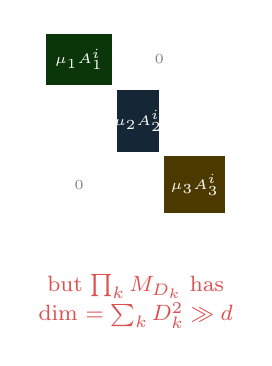
\begin{tikzpicture}[scale=0.6]
  \draw[white,thick] (0,0) rectangle (4,4);
  \fill[leangreen!30!black] (0.1,2.8) rectangle (1.5,3.9);
  \fill[leanblue!30!black] (1.6,1.4) rectangle (2.5,2.7);
  \fill[amber!30!black] (2.6,0.1) rectangle (3.9,1.3);
  \node[white,font=\tiny\bfseries] at (0.8,3.35) {$\mu_1 A_1^i$};
  \node[white,font=\tiny\bfseries] at (2.05,2.05) {$\mu_2 A_2^i$};
  \node[white,font=\tiny\bfseries] at (3.25,0.7) {$\mu_3 A_3^i$};
  \node[font=\tiny,gray] at (2.5,3.35) {$0$};
  \node[font=\tiny,gray] at (0.8,0.7) {$0$};
  \node[below=0.2cm,font=\footnotesize,white] at (2,0) {$\pi_A(i)$ has rank $\leq d$};
  \node[below=0.6cm,font=\footnotesize,softred] at (2,0) {but $\prod_k M_{D_k}$ has};
  \node[below=0.95cm,font=\footnotesize,softred] at (2,0) {dim $= \sum_k D_k^2 \gg d$};
\end{tikzpicture}
\end{center}
\end{columns}

\vspace{0.3em}
\notproved{Pi-tensors don't span the product algebra; cannot build the linear extension directly.}
\end{frame}

%======================================================================
% SLIDE 13 - Summary of Failed Approaches
%======================================================================
\begin{frame}{Summary: Why Every Algebraic Approach Fails}
\vspace{-0.3em}
\begin{center}
\renewcommand{\arraystretch}{1.35}
{\small
\begin{tabular}{>{\raggedright}p{3.2cm} >{\raggedright}p{4.5cm} >{\raggedright\arraybackslash}p{4.2cm}}
\hline
\textbf{Approach} & \textbf{Core idea} & \textbf{Why it fails} \\
\hline
\textcolor{softred}{Vandermonde across $N$} &
Fix $\sigma$, vary $N$ &
$\sigma : \mathrm{Fin}\,N \to \mathrm{Fin}\,d$ changes type \\[0.1em]

\textcolor{softred}{Word repetition $w^m$} &
Repeated word gives $\tr(M_k^m)$ &
$\tr(M_k^m)$ depends on $m$ \\[0.1em]

\textcolor{softred}{Padding with letter $j$} &
Prepend $p$ copies of $j$ &
$A_k(j)^p$ varies with $p$ \\[0.1em]

\textcolor{softred}{Induction on $N$} &
Bootstrap from small sizes &
No recursion: $\delta(N{+}1)$ $\not\leftarrow$ $\delta(N)$ \\[0.1em]

\textcolor{softred}{Induction on $r$} &
Reduce blocks one at a time &
Step requires the very separation we seek \\[0.1em]

\textcolor{softred}{Direct Pi construction} &
Build $T$ on $\prod M_{D_k}$ directly &
Pi-tensors don't span product algebra \\
\hline
\end{tabular}}
\end{center}

\vspace{0.5em}
\begin{center}
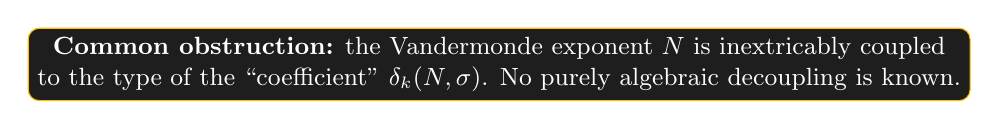
\begin{tikzpicture}
\node[rectangle,rounded corners,draw=amber,fill=cardbg,text=white,
  font=\small,align=center,minimum width=10.5cm,minimum height=0.7cm] {
  \textbf{Common obstruction:} the Vandermonde exponent $N$ is inextricably coupled\\
  to the type of the ``coefficient'' $\delta_k(N,\sigma)$. No purely algebraic decoupling is known.
};
\end{tikzpicture}
\end{center}
\end{frame}

%======================================================================
% SLIDE 14 - What the Physics Paper Does (Part 1)
%======================================================================
\begin{frame}{What the Physics Paper Does: Transfer Operators}
\vspace{-0.3em}
{\small In arXiv:2011.12127, \S IV, the separation uses the \textbf{transfer operator} (quantum channel):}
\[
\mathcal{E}_A(\rho) = \sum_{i=1}^d A^i \rho (A^i)^\dagger
\]

\vspace{-0.2em}
\begin{columns}[T]
\column{0.52\textwidth}
{\small\textbf{Key properties (physics):}}
\begin{enumerate}\itemsep0.15em
  \item {\small $\mathcal{E}_A$ is a \textbf{completely positive} (CP) map}
  \item {\small When $A$ is injective: $\mathcal{E}_A$ has a \textbf{unique} fixed point $\Lambda > 0$ (the steady state)}
  \item {\small $\mathcal{E}_A$ has \textbf{spectral gap}: all other eigenvalues have $|\lambda| < \rho(\mathcal{E}_A)$}
  \item {\small For the block-diagonal tensor: $\mathcal{E}_{\text{block}}$ decomposes into block transfer operators}
\end{enumerate}

\column{0.44\textwidth}
\begin{center}
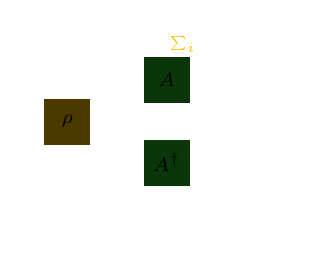
\begin{tikzpicture}[scale=0.7]
% Transfer operator diagram
\node[rectangle,draw=white,fill=leangreen!30!black,minimum size=0.6cm,
  font=\scriptsize\bfseries] (A1) at (0,0) {$A$};
\node[rectangle,draw=white,fill=leangreen!30!black,minimum size=0.6cm,
  font=\scriptsize\bfseries] (A2) at (0,-1.5) {$A^\dagger$};
\node[rectangle,draw=white,fill=amber!30!black,minimum size=0.6cm,
  font=\scriptsize\bfseries] (rho) at (-1.8,-0.75) {$\rho$};
% Wires
\draw[-,white,thick] (A1.west) -- (rho.north east);
\draw[-,white,thick] (A2.west) -- (rho.south east);
\draw[-,white,thick] (A1.north) -- ++(0,0.4) -- ++(1.2,0) -- ++(0,-1.15)
  -- (A2.north);
\draw[-,white,thick] (A1.east) -- ++(0.6,0);
\draw[-,white,thick] (A2.east) -- ++(0.6,0);
\node[font=\scriptsize,white,right] at (0.7,-0.3) {output};
\node[font=\scriptsize,white,right] at (0.7,-1.2) {output};
\node[font=\tiny,amber] at (0.3,0.65) {$\sum_i$};
% Label
\node[font=\scriptsize,white] at (-0.5,-2.5) {Transfer operator $\mathcal{E}_A$};
\end{tikzpicture}
\end{center}
\end{columns}

\vspace{0.3em}
{\small\textbf{The key insight:} As $N \to \infty$, the dominant block ($|\mu_k|$ largest) dominates the sum $\sum_k \mu_k^N \cdot V_k^{(N)}$. The spectral gap ensures exponential decay of subdominant contributions. Iterating, each block can be extracted.}
\end{frame}

%======================================================================
% SLIDE 15 - What the Physics Paper Does (Part 2)
%======================================================================
\begin{frame}{What the Physics Paper Does: Quantum Perron--Frobenius}
\vspace{-0.3em}
\begin{columns}[T]
\column{0.50\textwidth}
{\small\textbf{The argument in the paper:}}
\begin{enumerate}\itemsep0.15em
  \item {\small The transfer operator $\mathcal{E}_A$ for an injective MPS tensor has a \textbf{unique maximal eigenvalue} $\lambda = 1$ (after normalization)}
  \item {\small The corresponding eigenvector $\Lambda > 0$ is the \textbf{unique positive-definite} fixed point}
  \item {\small As $N \to \infty$:
  $ \tr(A^{i_1} \cdots A^{i_N}) \sim \lambda^N \cdot \tr(\Lambda \cdot A^{i_1} \cdots)$}
  \item {\small The block with largest $|\mu_k|$ dominates; subtract it off and repeat}
\end{enumerate}

\column{0.46\textwidth}
{\small\textbf{What this requires:}}
\begin{itemize}\itemsep0.1em
  \item[\textcolor{softred}{$\boldsymbol{\times}$}] {\small CP maps on $M_D(\mathbb{C})$}
  \item[\textcolor{softred}{$\boldsymbol{\times}$}] {\small Perron--Frobenius for positive maps}
  \item[\textcolor{softred}{$\boldsymbol{\times}$}] {\small Spectral theory for superoperators}
  \item[\textcolor{softred}{$\boldsymbol{\times}$}] {\small Convergence of $\mathcal{E}_A^n(\rho) \to \Lambda$}
  \item[\textcolor{softred}{$\boldsymbol{\times}$}] {\small Asymptotic expansion of $\tr(M^n)$}
\end{itemize}

\vspace{0.3em}
{\small \textcolor{softred}{\textbf{None of this is in Mathlib v4.27.0.}}}
\end{columns}

\vspace{0.3em}
\begin{center}
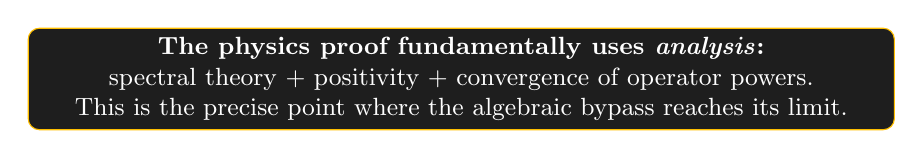
\begin{tikzpicture}
\node[rectangle,rounded corners,draw=amber,fill=cardbg,text=white,
  font=\small,align=center,minimum width=11cm,minimum height=0.9cm] {
  \textbf{The physics proof fundamentally uses \emph{analysis}:}\\
  spectral theory + positivity + convergence of operator powers.\\
  This is the precise point where the algebraic bypass reaches its limit.
};
\end{tikzpicture}
\end{center}
\end{frame}

%======================================================================
% SLIDE 16 - What Vandermonde Tools We DO Have
%======================================================================
\begin{frame}[fragile]{What We \emph{Can} Prove: Vandermonde at Fixed Size}
\vspace{-0.5em}
{\small Our formalization \emph{does} contain Vandermonde tools, but they work at a \textbf{fixed} system size:}

\vspace{0.1em}
\begin{lstlisting}[basicstyle=\ttfamily\fontsize{5}{6.5}\selectfont\color{white}]
-- Vandermonde separation for scalar coefficients (BasisNormal.lean)
theorem vandermonde_separation (C : CanonicalForm d)
    (h(*@$\mu$@*) : Function.Injective C.(*@$\mu$@*))
    (c : Fin C.numBlocks (*@$\to$@*) (*@$\mathbb{C}$@*))
    (hc : (*@$\forall$@*) N : Fin C.numBlocks,
      ((*@$\sum$@*) k, c k * (C.(*@$\mu$@*) k) ^ (N : (*@$\mathbb{N}$@*))) = 0) :
    c = 0

-- Function-valued Vandermonde (BasisNormal.lean)
theorem vandermonde_separation_fun {n : (*@$\mathbb{N}$@*)} {(*@$\alpha$@*) : Type*}
    ((*@$\mu$@*) : Fin n (*@$\to$@*) (*@$\mathbb{C}$@*)) (h(*@$\mu$@*) : Function.Injective (*@$\mu$@*))
    (v : Fin n (*@$\to$@*) (*@$\alpha$@*) (*@$\to$@*) (*@$\mathbb{C}$@*))
    (hv : (*@$\forall$@*) i : Fin n, (*@$\forall$@*) a : (*@$\alpha$@*),
      ((*@$\sum$@*) j, v j a * (*@$\mu$@*) j ^ (i : (*@$\mathbb{N}$@*))) = 0) :
    v = 0
\end{lstlisting}

\vspace{0.05em}
{\small\textbf{These apply when:} the ``coefficient'' $v_k$ is \textbf{independent of} the Vandermonde index $N$.}

\vspace{0.15em}
{\small\textbf{The gap is precisely:} our $\delta_k(N, \sigma)$ \emph{does} depend on $N$, which serves double duty as the Vandermonde exponent and the configuration space size.}

\vspace{0.1em}
{\small\proved{162 lines of Vandermonde infrastructure in \texttt{BasisNormal.lean}}\quad\proved{Used in \texttt{FundamentalTheoremMulti.lean}}}
\end{frame}

%======================================================================
% SLIDE 17 - The Exact Shape of the Obstacle
%======================================================================
\begin{frame}{The Exact Shape of the Obstacle}
\vspace{-0.5em}
{\small\textbf{Abstracting the problem:}
Let $V_k : \mathbb{N} \to \mathcal{H}_\bullet$ where $\mathcal{H}_N = (\mathrm{Fin}\,N \to \mathrm{Fin}\,d) \to \mathbb{C}$ is the ``state space at size $N$''.}

\vspace{0.1em}
\begin{center}
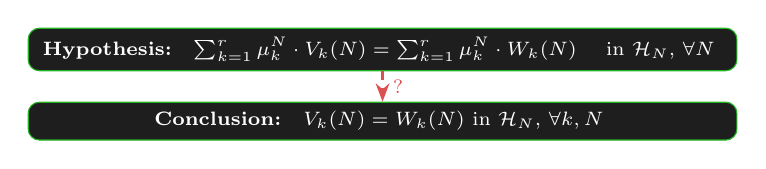
\begin{tikzpicture}[scale=0.7]
\node[rectangle,rounded corners,draw=leangreen,fill=cardbg,text=white,
  font=\scriptsize,align=left,minimum width=9cm] (hyp) at (0,1.3) {
  \textbf{Hypothesis:}\quad $\sum_{k=1}^r \mu_k^N \cdot V_k(N) = \sum_{k=1}^r \mu_k^N \cdot W_k(N)$
  \quad in $\mathcal{H}_N$,  $\forall N$
};
\node[rectangle,rounded corners,draw=leangreen,fill=cardbg,text=white,
  font=\scriptsize,align=left,minimum width=9cm] (conc) at (0,0) {
  \textbf{Conclusion:}\quad $V_k(N) = W_k(N)$ in $\mathcal{H}_N$,  $\forall k, N$
};
\draw[-{Stealth},softred,thick,dashed] (hyp) -- node[right,font=\scriptsize,softred]{?} (conc);
\end{tikzpicture}
\end{center}

\vspace{-0.2em}
{\small This is \textbf{not} a standard Vandermonde problem because $V_k(N)$ and $V_k(N')$ live in \emph{different} vector spaces for $N \neq N'$. It is a problem about a \textbf{graded family} of equations.}

\vspace{0.15em}
{\small\textbf{What makes it true} (in the MPS context):}
\vspace{-0.2em}
\begin{itemize}\itemsep0em
  \item {\small The maps $N \mapsto V_k(N)$ are not arbitrary --- they arise from \textbf{matrix traces}}
  \item {\small The transfer operator $\mathcal{E}_{A_k}$ governs the asymptotic behavior of $V_k(N)$ as $N \to \infty$}
  \item {\small The spectral gap of $\mathcal{E}_{A_k}$ provides exponential convergence, allowing block extraction}
\end{itemize}
\vspace{-0.1em}
{\small The truth depends on the \textbf{analytic structure} of MPVs, not just their algebraic properties.}
\end{frame}

%======================================================================
% SLIDE 18 - Path Forward: What Mathlib Needs
%======================================================================
\begin{frame}{Path Forward: What Mathlib Would Need}
\vspace{-0.3em}
\begin{columns}[T]
\column{0.48\textwidth}
{\small\textbf{\textcolor{softred}{Missing from Mathlib:}}}
\begin{enumerate}\itemsep0.15em
  \item {\small\textbf{Completely positive maps}\\
  {\scriptsize $C^*$-algebras exist in Mathlib, but CP maps, Stinespring, and Kraus representations do not.}}
  \item {\small\textbf{Perron--Frobenius for positive maps}\\
  {\scriptsize The non-negative matrix PF theorem is partially there. The $C^*$ version is missing entirely.}}
  \item {\small\textbf{Spectral theory for finite-dim operators}\\
  {\scriptsize Eigenvalue theory is available, but the connection to iterated powers $\mathcal{E}^n \to$ projection is not.}}
  \item {\small\textbf{Asymptotic expansion of $\tr(M^n)$}\\
  {\scriptsize Needs Jordan normal form or functional calculus.}}
\end{enumerate}

\column{0.48\textwidth}
{\small\textbf{\textcolor{leangreen}{What exists / is close:}}}
\begin{itemize}\itemsep0.15em
  \item {\small Spectral theory for normal operators (partially in Mathlib)}
  \item {\small Jordan blocks (not in Mathlib, but defined in some projects)}
  \item {\small Polynomial eigenvalue characterization}
  \item {\small Finite-dim $\Rightarrow$ finitely many eigenvalues}
\end{itemize}

\vspace{0.5em}
\begin{center}
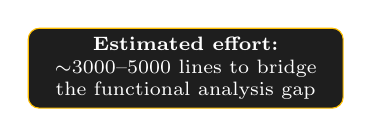
\begin{tikzpicture}
\node[rectangle,rounded corners,draw=amber,fill=cardbg,text=white,
  font=\scriptsize,align=center,minimum width=4cm,minimum height=0.7cm] {
  \textbf{Estimated effort:}\\
  $\sim$3000--5000 lines to bridge\\
  the functional analysis gap
};
\end{tikzpicture}
\end{center}
\end{columns}
\end{frame}

%======================================================================
% SLIDE 19 - Alternative Algebraic Approaches
%======================================================================
\begin{frame}{Alternative Approaches Still Unexplored}
\vspace{-0.3em}
{\small Could one avoid transfer operators entirely? Some speculative directions:}

\vspace{0.3em}
\begin{columns}[T]
\column{0.48\textwidth}
{\small\textbf{\textcolor{amber}{1.\ Generating functions.}}}\\[0.1em]
{\scriptsize Define $F_k(z) = \sum_{N \geq 0} V_k(N) \cdot z^N$ as a formal power series. The hypothesis becomes $\sum_k F_k(\mu_k z) = \sum_k G_k(\mu_k z)$. Can formal power series identity + radius of convergence arguments help?\\[0.1em]
\textbf{Obstacle:} $V_k(N)$ lives in varying spaces.}

\vspace{0.3em}
{\small\textbf{\textcolor{amber}{2.\ Newton's identities.}}}\\[0.1em]
{\scriptsize For the word repetition approach: $\tr(M^m)$ are the power sums of eigenvalues. Newton's identities recover the characteristic polynomial, and hence the eigenvalues, from $\{\tr(M^m)\}_{m=1}^{D}$.\\[0.1em]
\textbf{Obstacle:} Need Newton's identities in Mathlib, plus eigenvalue extraction.}

\column{0.48\textwidth}
{\small\textbf{\textcolor{amber}{3.\ Symbolic evaluation.}}}\\[0.1em]
{\scriptsize Instead of scalar MPVs, work with \emph{formal matrix products}: define a symbolic evaluation ring where $\mathrm{eval}(A_k, \sigma) \in M_{D_k}(\mathbb{C})$ is the formal product before taking trace. The trace coupling might decouple at the matrix level.\\[0.1em]
\textbf{Obstacle:} Unclear how to state the right hypothesis.}

\vspace{0.3em}
{\small\textbf{\textcolor{amber}{4.\ Density argument.}}}\\[0.1em]
{\scriptsize The set of configurations $\{\sigma : \mathrm{Fin}\,N \to \mathrm{Fin}\,d\}$ for varying $N$ generates, in some sense, all of $M_{D_k}(\mathbb{C})$ via the injective tensor. Perhaps a careful spanning argument over \emph{all sizes simultaneously} could work.\\[0.1em]
\textbf{Obstacle:} Not clear how to formalize.}
\end{columns}
\end{frame}

%======================================================================
% SLIDE 20 - The Open Question
%======================================================================
\begin{frame}{The Open Question}
\vspace{-0.2em}
\begin{center}
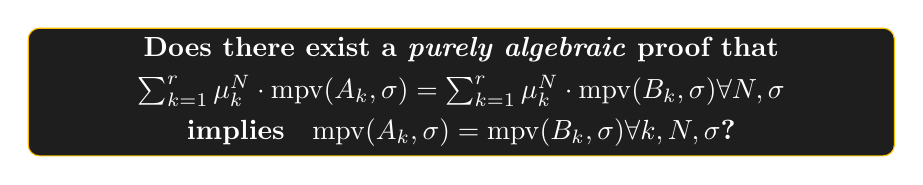
\begin{tikzpicture}
\node[rectangle,rounded corners,draw=amber,fill=cardbg,text=white,
  font=\normalsize,align=center,minimum width=11cm,minimum height=1.6cm] {
  \textbf{Does there exist a \emph{purely algebraic} proof that}\\[0.3em]
  $\sum_{k=1}^r \mu_k^N \cdot \mathrm{mpv}(A_k, \sigma) = \sum_{k=1}^r \mu_k^N \cdot \mathrm{mpv}(B_k, \sigma)  \forall N, \sigma$\\[0.3em]
  \textbf{implies}\quad $\mathrm{mpv}(A_k, \sigma) = \mathrm{mpv}(B_k, \sigma)  \forall k, N, \sigma$\textbf{?}
};
\end{tikzpicture}
\end{center}

\vspace{0.3em}
\begin{columns}[T]
\column{0.48\textwidth}
{\small\textbf{Arguments it might exist:}}
\begin{itemize}\itemsep0.1em
  \item {\small The statement is purely algebraic}
  \item {\small All objects are finite-dimensional}
  \item {\small The MPS structure is highly constrained}
  \item {\small Injectivity is a strong condition}
\end{itemize}

\column{0.48\textwidth}
{\small\textbf{Arguments it might not:}}
\begin{itemize}\itemsep0.1em
  \item {\small All known proofs use spectral theory}
  \item {\small The graded nature seems essential}
  \item {\small The coupling of $N$ with $\sigma$-type is structural}
  \item {\small Even the paper uses $N \to \infty$ limits}
\end{itemize}
\end{columns}

\vspace{0.5em}
{\small\textbf{For the formalization:} We have documented this gap transparently. The final theorems take per-block \texttt{SameMPV} as a hypothesis, which is exactly the setting where two canonical forms with identified block correspondence are given. The gap is the bridge from global to local MPV equality.}

\vspace{0.3em}
{\small\textbf{Either} a purely algebraic proof is found (closing the gap in $\sim$100--200 lines of Lean), \textbf{or} Mathlib's functional analysis library grows to support the spectral argument ($\sim$3000--5000 lines).}
\end{frame}

%======================================================================
% SLIDE 21 - Current Status and What Remains
%======================================================================
\begin{frame}{Current Status: Where the Gap Sits}
\vspace{-0.5em}
\begin{center}
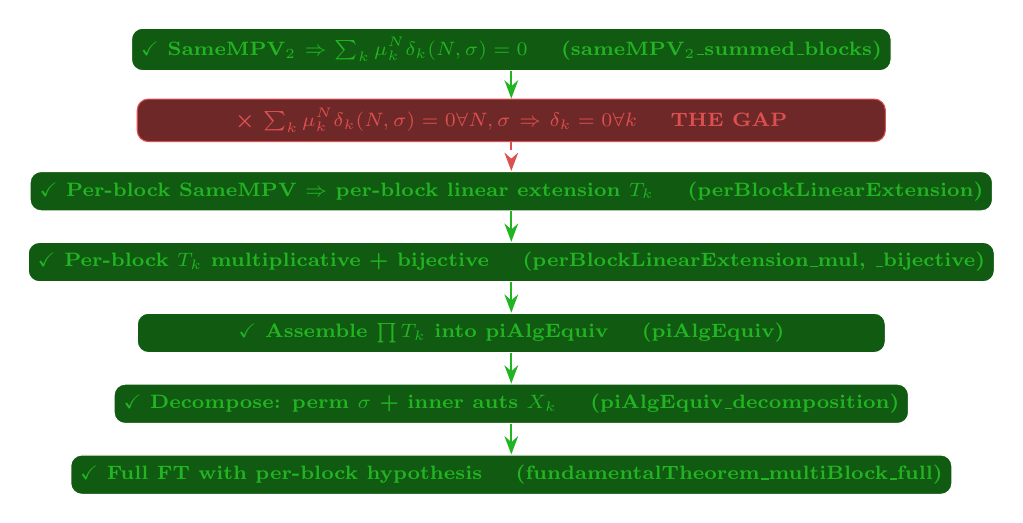
\begin{tikzpicture}[xscale=0.95,
  box/.style={rectangle,rounded corners,draw=white,text=white,
    font=\scriptsize\bfseries,minimum width=9.5cm,minimum height=0.5cm},
  done/.style={fill=leangreen!50!black},
  gap/.style={fill=softred!50!black,draw=softred}
]
\node[box,done] (s1) at (0,4.8) {\proved{SameMPV${}_2$ $\Rightarrow$ $\sum_k \mu_k^N \delta_k(N,\sigma) = 0$ \quad(sameMPV${}_2$\_summed\_blocks)}};
\node[box,gap] (s2) at (0,3.9) {\notproved{$\sum_k \mu_k^N \delta_k(N,\sigma) = 0 \forall N,\sigma$ $\Rightarrow$ $\delta_k = 0 \forall k$ \quad\textbf{THE GAP}}};
\node[box,done] (s3) at (0,3.0) {\proved{Per-block SameMPV $\Rightarrow$ per-block linear extension $T_k$ \quad(perBlockLinearExtension)}};
\node[box,done] (s4) at (0,2.1) {\proved{Per-block $T_k$ multiplicative + bijective \quad(perBlockLinearExtension\_mul, \_bijective)}};
\node[box,done] (s5) at (0,1.2) {\proved{Assemble $\prod T_k$ into piAlgEquiv \quad(piAlgEquiv)}};
\node[box,done] (s6) at (0,0.3) {\proved{Decompose: perm $\sigma$ + inner auts $X_k$ \quad(piAlgEquiv\_decomposition)}};
\node[box,done] (s7) at (0,-0.6) {\proved{Full FT with per-block hypothesis \quad(fundamentalTheorem\_multiBlock\_full)}};

\draw[-{Stealth},leangreen,thick] (s1) -- (s2);
\draw[-{Stealth},softred,thick,dashed] (s2) -- (s3);
\draw[-{Stealth},leangreen,thick] (s3) -- (s4);
\draw[-{Stealth},leangreen,thick] (s4) -- (s5);
\draw[-{Stealth},leangreen,thick] (s5) -- (s6);
\draw[-{Stealth},leangreen,thick] (s6) -- (s7);
\end{tikzpicture}
\end{center}
\vspace{-0.3em}
{\small \textbf{Everything above and below the gap is machine-verified.} The gap is a single logical step: separating the weighted sum into per-block equalities.}
\end{frame}

%======================================================================
% SLIDE 22 - Thank You
%======================================================================
\begin{frame}
\begin{center}
\vspace{0.5em}
\Huge\textbf{\textcolor{leangreen}{Thank You!}}

\vspace{0.8em}
\LARGE Questions?

\vspace{1em}
\large\texttt{github.com/LionSR/MPSLean}

\vspace{0.4em}
\normalsize Built on Lean 4 + Mathlib v4.27.0

\vspace{0.3em}
{\small Reference: Cirac, P\'erez-Garc\'ia, Schuch \& Verstraete  $\cdot$  \texttt{arXiv:2011.12127}}

\vspace{0.6em}
\textcolor{leangreen}{\textbf{2792 lines\quad$\cdot$\quad 16 modules\quad$\cdot$\quad 0 sorries\quad$\cdot$\quad 0 axioms}}

\vspace{0.5em}

\begin{tikzpicture}
\node[rectangle,rounded corners,draw=amber,fill=cardbg,text=white,
  font=\small,align=center,minimum width=8cm,minimum height=0.7cm] {
  \textbf{One gap remains:} SameMPV${}_2$ $\Rightarrow$ per-block SameMPV\\
  Requires spectral theory not yet in Mathlib --- or a new algebraic proof
};
\end{tikzpicture}
\end{center}
\end{frame}

\end{document}